\documentclass[a4paper]{article}
\usepackage[latin1]{inputenc}
\usepackage{graphicx}
\usepackage{array}
\usepackage{amsmath}
\newcommand{\transp}{\top}

\usepackage{caption}
\usepackage{subcaption}

\setlength{\parskip}{2ex}

\begin{document}


\title{Independent Study Report - CB + DMPs}
\author{Francisco M. Garcia}
%\date{}

\maketitle


\section{Introduction}

\indent \indent In this independent study, I focused my attention to two related approaches to motor control: Control Basis (CB) and Dynamic Movement Primitives (DMPs). CB provides a way of generating complex movement from a sequential composition of simple primitives, while DMPs is a parametric model that allows the reproduction and generalization of demonstrations. \\
\indent One of the limitations of CB is that it requires convergence of a given component before the next one can begin to execute, which leads to slow execution with little generalization capabilities. By using these movements as demonstrations, DMPs could reproduce these controllers with a high degree of flexibility. In this work, I study the feasibility of a hybrid approach in which CB provides an unsupervised method for generating movements and DMPs generalize and improves the demonstrations.

\section{Control Basis}

\indent \indent The Control Basis is a closed-loop method that allows to create complex behavior by combining feedback control elements. In this framework, movements are generated by taking into account the set of available input resources $\sigma$ (sensors), and output resources $\tau$ (actuators). Every action is limited by a "subject to" constraint, which restricts the control actions such that new actions do not draw the system away from achieving higher priority objectives. A control policy, then, is a sequence of controllers that is learned via RL subject to input and output resources.    

\section{Dynamic Movement Primitives}

\indent \indent Dynamic Movement Primitives (DMPs) provide a general approach for learning robotic motor skill from demonstration. Given a sample trajectory with start state $x_0$ and goal state $g$, a DMP generates a trajectory by integrating the following equations:

$$
\tau \dot{v} = K(g - x) - Dv - K(g - x_0) s + Kf(s)
$$
$$
\tau \dot{x} = v
$$

In these equations, $\tau$ refers to a time scaling term, $K$ and $D$ refer on system specific constant that work as in a PD controller and $f(s)$ corresponds to a non-linear function composed of several Gaussian basis functions:

$$
f(s) = \frac{\sum_i w_i \psi_i(s) s }{\sum_i \psi_i(s)}
$$

where $\psi_i(s) = \exp(-h_i(s-c_i)^2)$ are the basis functions with center $c_i$ and width $h_i$. $w_i$ are the parameters to be found to minimize the objective function J. \\
\indent The variable $s$ is a phase variable which encompasses the duration of the trajectory and monotonically decreases from 1 to 0. This variable obtained by the canonical system:
$$
\tau \dot{s} = -\alpha s
$$
 
When observing a demonstration, a movement $x(t)$ is recorded and from that its derivative $v(t)$ and $\dot{v}$ are obtained. Using this, we can compute the target function:
$$
f_{target}(s) = \frac{\tau \dot{v} + Dv}{K} - (g - x) + (g - x_0) s
$$ 

and solve the objective function $J = \sum_s (f_{target}(s) - f(s))^2$ via gradient descent or least-squares. \\
\indent Once trained, a new trajectory can be generated by setting $s$ to 1, updating the positions and velocities and integrating the canonical system to obtained the new $s$.

Figure \ref{fig:test} shows the plot of DMPs for a 2-link robotic arm simulator. The x-axis is time measured in seconds, while the y-axis measures the angular position in radians. The line in red is the trajectory of the demonstration, while the line in blue is the approximation generated from the DMP. In this case, the DMPs are set to the same initial and goal positions, so as to recreate the same movement.  
 
 
\begin{figure}
\centering
\begin{subfigure}{.5\textwidth}
  \centering
  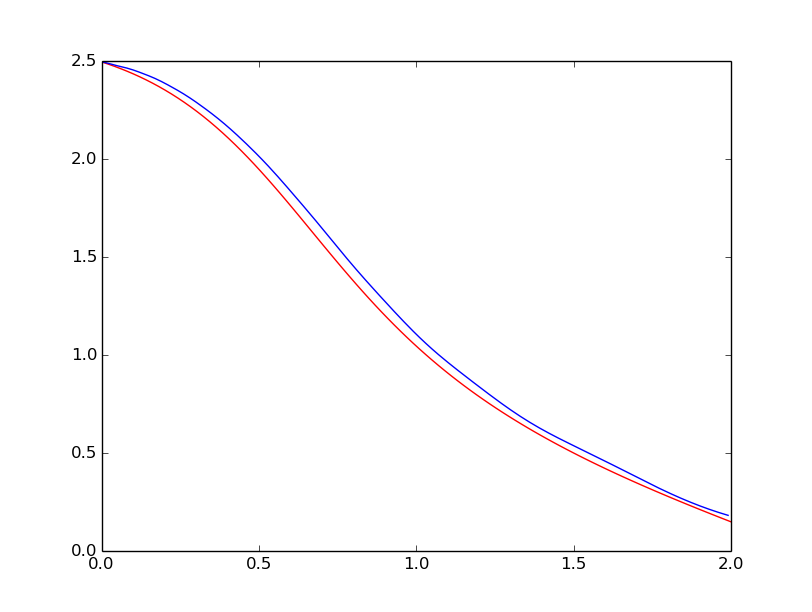
\includegraphics[width=.8\linewidth]{figure_1.png}
  \caption{DMP for joint 1}
  \label{fig:sub1}
\end{subfigure}%
\begin{subfigure}{.5\textwidth}
  \centering
  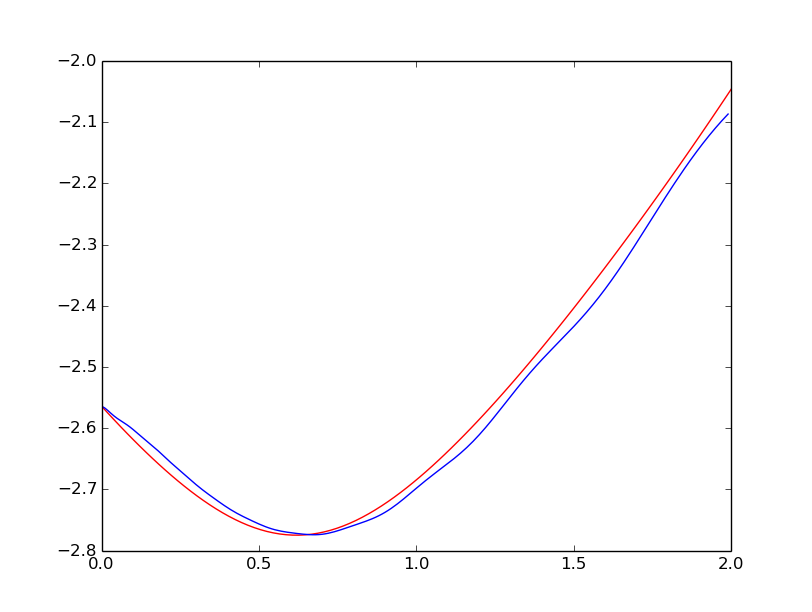
\includegraphics[width=.8\linewidth]{figure_2.png}
  \caption{DMP for joint 2}
  \label{fig:sub2}
\end{subfigure}
\caption{Plot of demonstrations and their corresponding DMP}
\label{fig:test}
\end{figure}

\section{Combining CB and DMPs}

\indent \indent As discussed in previous sections, the Control Basis and DMPs provide the potential to a hybrid approach where CB generate demonstrations without the need of human supervision and the DMPs generalize that movement in space and time. In this section, I show some preliminary results showcasing the feasibility of combining these methods. \\

\indent Figure \ref{fig:ubot} shows the trajectory of 2 joints for a simulated task on the uBot. The task consists of picking up a box, lifting it and putting it back down. As we can see, even though the trajectory of the DMP learned in \ref{fig:cbdmp2} is a similar recreation of the demonstration, the trajectory in \ref{fig:cbdmp1} is a much smoother trajectory than the one demonstrated. 


\begin{figure}
\centering
\begin{subfigure}{.5\textwidth}
  \centering
  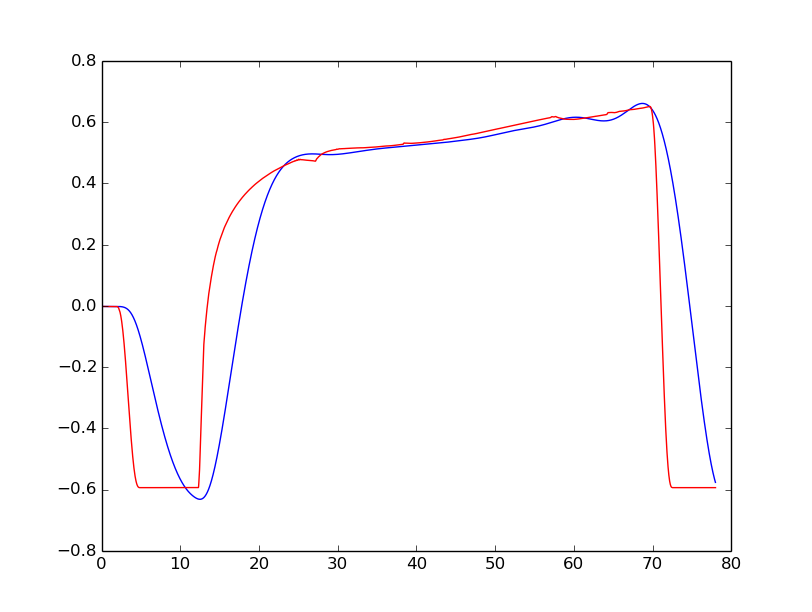
\includegraphics[width=.8\linewidth]{cb_dmp1.png}
  \caption{Trajectory for right shoulder joint.}
  \label{fig:cbdmp1}
\end{subfigure}%
\begin{subfigure}{.5\textwidth}
  \centering
  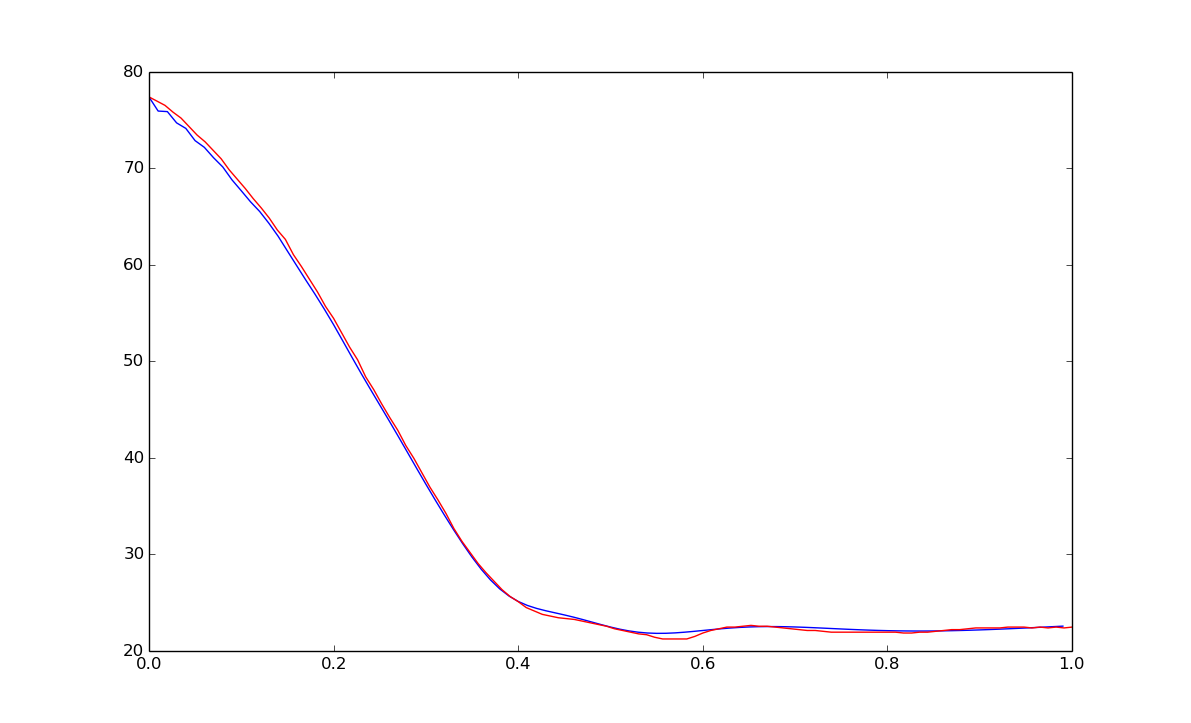
\includegraphics[width=.8\linewidth]{cb_dmp2.png}
  \caption{Trajectory for right elbow joint.}
  \label{fig:cbdmp2}
\end{subfigure}
\caption{Plot of uBot task trajectories for picking up a box.}
\label{fig:ubot}
\end{figure}
 
 
Figure \ref{fig:ubot_gen} shows the generalization capabilities of the Control Basis and DMP hybrid framework. Figure \ref{fig:cbdmp3} shows the demonstration for one of the joints in the aforementioned task, where the goal position has been offset by 5 degrees from the original demonstration. Figure \ref{fig:cbdmp4} shows the plot of the demonstrated trajectories scaled in time. As we can see, both cases maintain the general shape of the demonstrated trajectory, while achieving different goals or time constraints.
 
 
\begin{figure}
\centering
\begin{subfigure}{.5\textwidth}
  \centering
  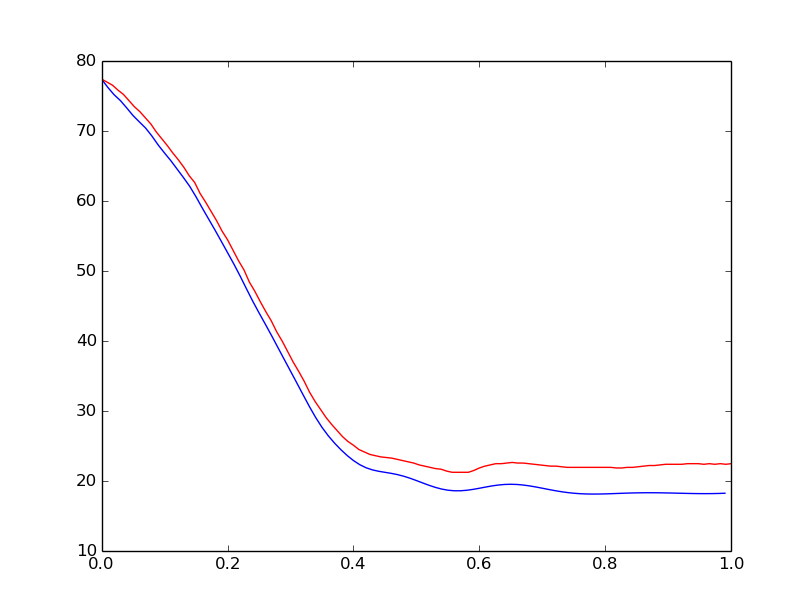
\includegraphics[width=.8\linewidth]{cb_dmp3.png}
  \caption{Generalization in joint space.}
  \label{fig:cbdmp3}
\end{subfigure}%
\begin{subfigure}{.5\textwidth}
  \centering
  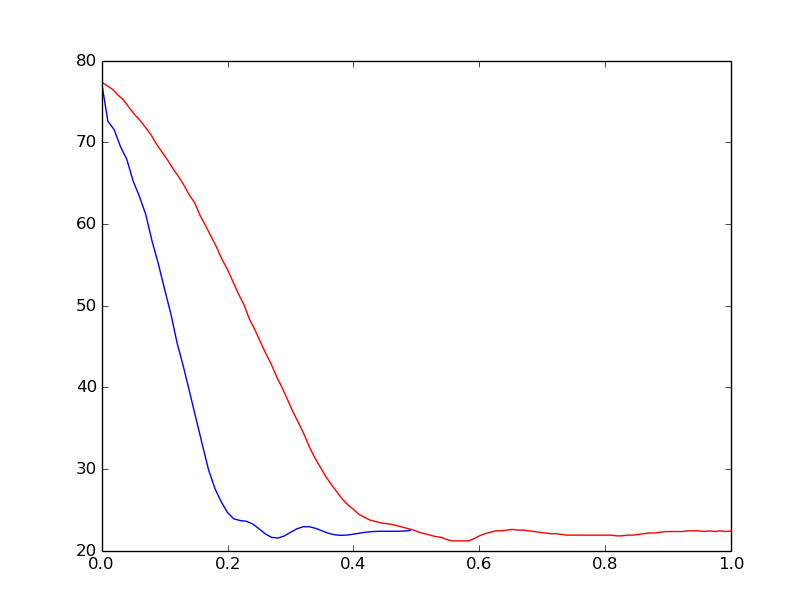
\includegraphics[width=.8\linewidth]{cb_dmp4.png}
  \caption{Generalization in time.}
  \label{fig:cbdmp4}
\end{subfigure}
\caption{Demonstration of generalization capabilities of CB+DMP.}
\label{fig:ubot_gen}
\end{figure}

\section{Future Directions}

In this study, I show a different approach to learning to learning movements without the need of human demonstration and control its ability to generalize to different locations and different execution times. Having shown that this framework is a viable alternative to current methodology opens the doors to several possibilities for further investigation. \\
\indent Some possible research directions to explore would be:
\begin{itemize}
	\item \textbf{Error Detection:} An interesting problem that arose as I was working on this study was, \textit{how can the system detect whether it is able to complete a movement or not?} The current solution I implemented keeps track of a history of the $k$ last errors. At each time step, $t$, the current state, $x_t$, of the system is evaluated against the desired state, $x'_t$. If $(|x_t - x'_t| - |x_{t-k} - x'_{t-k}|) > \epsilon$, where $\epsilon$ is some predefined threshold, and the error is non-decreasing between time $t-k$ and $t$, the system infers an obstacle is present and enters error handling mode. Effectively, this says that if between those two time periods, the error of the system is only increasing and goes beyond a certain point, it infers that there is some obstacle preventing it form making progress.
	
	\item \textbf{Error Correction:} Once an error is detected, there are several possibilities on how one could handle recovery. One approach is to increase the value of $s$ during the DMP execution, which in turn makes the system run "backwards" in time. That is, if the system is at $s_{t-k}$ when in state $x_{t-k}$ and at $s_t$ in state $x_t$, we can increase $s$ for $k$ steps such that $s_{t+k} = s_{t-k}$, taking the system to state $x_{t+k} = x{t-k}$. This would let us go back to a point before the error was encounter and either execute a different DMP or adjust the current one with the knowledge that there must be an obstacle present. \\
	\indent An alternative approach could make use of the contact detected and instead of backtracking to a point before coming in contact with an obstacle, follow a direction perpendicular to the force vector such as to move around the obstacle. 
	
	\item \textbf{Achieving Subgoals:} It is possible to execute a DMP to completion without achieving the desired result. Consider the task of a robot grabbing a box a lifting it; small errors could be not large enough to be detected as significant errors and the DMP would make corrections during execution. However, these small errors could cause the robot to miss grabbing the box and still execute a similar movement that did not accomplish this sub-goal. An interesting question would be, how can the system automatically detect where these subgoals lay and enforce their completion during a movement execution.
	
	\item \textbf{Optimizing Parameters:} Once a DMP is learned, how can the trajectory be modified such that the movement is qualitative similar but optimizes some criterion (e.g. energy)?

\end{itemize}
  
 
\end{document}